\documentclass[12pt, a4paper]{memoir} % for a short document
\usepackage[french,english]{babel}

\usepackage [vscale=0.76,includehead]{geometry}                % See geometry.pdf to learn the layout options. There are lots.
%\geometry{a4paper}                   % ... or a4paper or a5paper or ... 
%\geometry{landscape}                % Activate for for rotated page geometry
%\OnehalfSpacing
% \setSingleSpace{1.05}
%\usepackage[parfill]{parskip}    % Activate to begin paragraphs with an empty line rather than an indent


%===================================== packages
\usepackage{lipsum}
\usepackage{graphicx}
\usepackage{amsmath}
\usepackage{fullpage}
\usepackage{mathptmx} % font = times
\usepackage{helvet} % font sf = helvetica
\usepackage[latin1]{inputenc}
\usepackage{relsize}
\usepackage[T1]{fontenc}
\usepackage{tikz}
\usepackage{booktabs}
\usepackage{textcomp}%textquotesingle
\usepackage{multirow}
\usepackage{pgfplots}
\usepackage{url}
\usepackage{footnote}
\usepackage{subcaption}
\usepackage{amsfonts}
\usepackage{listings}
\usepackage{xcolor}
\usepackage{float}
\usepackage{wrapfig}

\definecolor{codegreen}{rgb}{0,0.6,0}
\definecolor{codegray}{rgb}{0.5,0.5,0.5}
\definecolor{codepurple}{rgb}{0.58,0,0.82}
\definecolor{backcolour}{rgb}{0.95,0.95,0.92}

\lstdefinestyle{mystyle}{
    backgroundcolor=\color{backcolour},   
    commentstyle=\color{codegreen},
    keywordstyle=\color{magenta},
    numberstyle=\tiny\color{codegray},
    stringstyle=\color{codepurple},
    basicstyle=\ttfamily\footnotesize,
    breakatwhitespace=false,         
    breaklines=true,                 
    captionpos=b,                    
    keepspaces=true,                 
    numbers=left,                    
    numbersep=5pt,                  
    showspaces=false,                
    showstringspaces=false,
    showtabs=false,                  
    tabsize=4
}

\lstset{style=mystyle}

\newcommand{\IFa}{\uparrow\mathrm{IF}}
\newcommand{\IFr}{\downarrow\mathrm{IF}}
\newcommand{\IDa}{\uparrow\mathrm{ID}}
\newcommand{\IDr}{\downarrow\mathrm{ID}}
\newcommand{\FUa}{\uparrow\mathrm{FU}}
\newcommand{\FUr}{\downarrow\mathrm{FU}}
\newcommand{\COM}{\mathrm{COM}}

%============================================
\usetikzlibrary{arrows,shapes,positioning,shadows,trees}
\makesavenoteenv{tabular}
\makesavenoteenv{table}
%==============================================
\def\checkmark{\tikz\fill[scale=0.4](0,.35) -- (.25,0) -- (1,.7) -- (.25,.15) -- cycle;}
%Style des têtes de section, headings, chapitre
\headstyles{komalike}
\nouppercaseheads
\chapterstyle{dash}
\makeevenhead{headings}{\sffamily\thepage}{}{\sffamily\leftmark} 
\makeoddhead{headings}{\sffamily\rightmark}{}{\sffamily\thepage}
\makeoddfoot{plain}{}{}{} % Pages chapitre. 
\makeheadrule{headings}{\textwidth}{\normalrulethickness}
%\renewcommand{\leftmark}{\thechapter ---}
\renewcommand{\chaptername}{\relax}
\renewcommand{\chaptitlefont}{ \sffamily\bfseries \LARGE}
\renewcommand{\chapnumfont}{ \sffamily\bfseries \LARGE}
\setsecnumdepth{subsection}


% Title page formatting -- do not change!
\pretitle{\HUGE\sffamily \bfseries\begin{center}} 
\posttitle{\end{center}}
\preauthor{\LARGE  \sffamily \bfseries\begin{center}}
\postauthor{\par\end{center}}
\newcommand{\jury}[1]{% 
\gdef\juryB{#1}} 
\newcommand{\juryB}{} 
\newcommand{\session}[1]{% 
\gdef\sessionB{#1}} 
\newcommand{\sessionB}{} 
\newcommand{\option}[1]{% 
\gdef\optionB{#1}} 
\newcommand{\optionB} {}

\usepackage{xcolor}
\newcommand{\TODO}[1]{\colorbox{red!30}{TODO: \textbf{#1}}}
% \newcommand{\TODO}[1]{}

\usepackage[most]{tcolorbox}
\newcounter{example}
\newtcolorbox{examplebox}[2][]{
    colback=gray!10,
    colframe=gray!80,
    boxrule=0.5pt,
    arc=3pt,
    left=6pt,
    right=6pt,
    top=4pt,
    bottom=4pt,
    fonttitle=\bfseries,
    title={Example~#2:~#1}
}
\newenvironment{example}[1][]{
    \refstepcounter{example}
    \begin{examplebox}[#1]{\theexample}
}{
    \end{examplebox}
}

\newcounter{assumption}
\newtcolorbox{assumptionbox}[2][]{
    colback=blue!5,
    colframe=blue!40,
    boxrule=0.5pt,
    arc=3pt,
    left=6pt,
    right=6pt,
    top=4pt,
    bottom=4pt,
    fonttitle=\bfseries,
    title={Assumption~#2:~#1}
}
\newenvironment{assumption}[1][]{
    \refstepcounter{assumption}
    \begin{assumptionbox}[#1]{\theassumption}
}{
    \end{assumptionbox}
}

\renewcommand{\maketitlehookd}{% 
\vfill{}  \large\par\noindent  
\begin{center}\juryB \bigskip\sessionB\end{center}
\vspace{-1.5cm}}
\renewcommand{\maketitlehooka}{% 
\vspace{-1.5cm}\noindent
\includegraphics[height=12ex]{pics/logo-uga.png}\hfill\raisebox{2ex}{
\includegraphics[height=14ex]{pics/logoINP.png}}\\
\bigskip
\begin{center} \large
Master of Science in Informatics at Grenoble \\
Master Informatique \\ 
Specialization \optionB  \end{center}\vfill}
% =======================End of title page formatting

\option{Parallel Computing and Distributed Systems} 
\title{Timing Anomaly through Branch Prediction} %\\\vspace{-1ex}\rule{10ex}{0.5pt} \\sub-title} 
\author{Andrei Ilin}
\date{Defense Date, 2025} % Delete this line to display the current date
\jury{
Research project performed at VERIMAG \\\medskip
Under the supervision of:\\
Lionel Rieg\\\medskip
Florian Brandner\\\medskip
Mihail Asavoae\\\medskip
% Defended before a jury composed of:\\
% Head of the jury\\
% Jury member 1\\
% Jury member 2\\
}
\session{June \hfill 2025}
\setcounter{tocdepth}{4}
\setcounter{secnumdepth}{4}

%%% BEGIN DOCUMENT
\begin{document}
\selectlanguage{English} % french si rapport en français
\frontmatter
\begin{titlingpage}
\maketitle
\end{titlingpage}

%\small
\setlength{\parskip}{-1pt plus 1pt}

\renewcommand{\abstracttextfont}{\normalfont}
\abstractintoc
\begin{abstract} 
In this report, we consider counter-intuitive timing anomalies (TAs) due to branch prediction in out-of-order (OoO) processor pipelines. A TA is a phenomenon when a local speedup in instruction execution leads to a global slowdown. We overview the existing TAs definitions and evaluate the applicability of the most promising one to branch prediction, using a novel ad-hoc model checking tool. Finally, we show that although the chosen definition adequately capture some TAs caused by branch prediction, its definition of causality cannot always capture the proper causality connections. This suggests that finding consistent TA definition encompassing branch prediction is still an open problem.

\end{abstract}
\abstractintoc

% \renewcommand\abstractname{Acknowledgement}
% \begin{abstract}
% I would like to express my sincere gratitude to .. for his invaluable assistance and comments in reviewing this report... 
% Good luck :) 
% \end{abstract}


\renewcommand\abstractname{R\'esum\'e}
\begin{abstract} \selectlanguage{French}
Dans ce rapport, nous \'etudions les anomalies temporelles contre-intuitives dues \`a la pr\'ediction de branchement dans les pipelines de processeurs \`a ex\'ecution dans le d\'esordre. Une TA est un ph\'enom\`ene o\`u une acc\'el\'eration locale de l'ex\'ecution d'une instruction conduit \`a un ralentissement global de l'ex\'ecution. Nous passons en revue les d\'efinitions existantes des TAs et \'evaluons l'applicabilit\'e de la plus prometteuse \`a la pr\'ediction de branchement, en utilisant un nouvel outil de model checking ad hoc. Enfin, nous montrons que, bien que la d\'efinition choisie capture correctement certaines TAs caus\'ees par la pr\'ediction de branchement, sa d\'efinition de la causalit\'e ne permet pas toujours de bien saisir les bons liens de causalit\'e. Cela sugg\`ere que concevoir une d\'efinition coh\'erente des TAs englobant la pr\'ediction de branchement reste un probl\`eme ouvert.
\end{abstract}
\selectlanguage{English}

\cleardoublepage

\tableofcontents* % the asterisk means that the table of contents itself isn't put into the ToC
\normalsize

\mainmatter
\SingleSpace
%==============================CHAPTERS==================
\chapter{Introduction}

For real time systems it is important to satisfy timing requirement, meaning that the time of program execution must be predictable. WCET analysis aims at giving an upper-bound of execution time. ...
Some text \cite{perais_increasing_2016}


\chapter{Background}

\section{Instruction Set architecture}

Instruction Set Architecture (ISA) defines the set of instructions and the registers on which they operate. Normally, the instruction operands are read from the registers and the execution result is stored there. ISA serves as an interface between software and actual hardware microarchitecture which implements the ISA. 

\TODO{what is ISA-state, instructions-granularity. ISA-level reigsters, mapping to real regs}

\section{Microarchitecture}

ISA defines binary format of instructions which are stored in memory and accessed by the processor through cache mechanisms, usually, fixed length instructions are used, while cariable-length also exist. (\TODO{add examples}). Processor is a cycled device that performs fetching instructions from memory and their subsequent execution, we call the microarchitectural state the state of all hardware registers of the processor. Unlike in ISA, states are defined at clock-cycle granularity, so an instruction takes several clock-cycles to finish. Different optimizations, such as pipelining, multiscalar execution, out-of-order execution and brach predictors (speculative execution).

\subsection{Processor Pipeline Stages}

Each instruction needs several microopererations to be executed: first, the instruction is to be loaded from memory, the operands need to be loaded from the registry. After that the instruction is executed during several cycles depending on its type (for example, multiplication is longer than addition). Due to the fact of isolation of those micropererations, it is possible to execute several instructions simultaneously: when instructions free its stage, next instruction enters it. This optimization, called pipelining, allows to increase the throughput of the processor.

\TODO{Is the word "microopererations" correct here?}

Several decompositions can exist for modern processors. Here we describe the 5 stages that can found in any processor and some of which may be further decomposed in more sophisticated architectures.

\subsubsection{Instruction Fetch (IF)}

As it was said before, the program instructions reside in global memory. This means that instructions access needs to be performed through memory hierarchy using program counter (PC) address. Often, a special instruction cache exists for accessing the program. IF stage is also responsible for updating PC to read the new instruction.

\subsubsection{Instruction Decode (ID)}

Once the instruction is fetched from memory, it exists in a processor in a packed binary format. This encoding includes the type of instruction as well as the registers it operates with. Decode stage loads the actual values from Physical Registry File (PRF) and propagates them to downstream pipeline stages. Sometimes the value can be obtained through bypass network before it appears in PRF.

\subsubsection{Execute (EX)}

EX stage computes the result of the operation. Several components may be responsible for performing different types of operations (for instance, different components for addition and multiplication). In this case IF stage emits control signals that determine the data path.

In case of memory or jump instruction the address is calculated.

The result of the computation is directly available to the ID stage via bypass network.

\subsubsection{Access Memory (MEM)}

This stage performs access to the global memory through memory hierarchy. If instruction is not a memory instruction, this stage is skipped.

\subsubsection{Commit (COM)}

The purpose of the last stage is to write the result of the instruction to PRF. Only after this the result is visible from ISA-state perspective.

\subsection{Restrictions}

The structure of the program imposes limitations on execution. Instruction may block each other thus stalling the pipeline. 

\subsubsection{Data Hazards}

There exist three types of register dependencies that may cause pipeline stall.

\textbf{Read-After-Write (RAW)} dependencies, also called as true data dependencies, arise when to perform one operation, the result of the other must be obtained. For example expression $(1 + 2 * 3)$ requires $(2 * 3)$ be calculated first, thus creating \textit{RAW}-dependency between multiplication and addition operations.

\textbf{Write-After-Write (WAW)} dependency happens when two instructions are writing to the same ISA-level register. The two writes must happen is instruction order.

\textbf{Write-after-Read (WAR)} dependency exists when the younger instruction aims at writing a value in the register which is to be read by an older instruction.

RAW-hazards are inevitable in any architecture. WAW and WAR dependencies do not exist in the model we described so far, by must be resolved in out-of-order pipeline.

\subsubsection{Control Hazards}

Fetching next instruction is possible only if the address of it is known. In case of branches, the next instruction address is not known until the branch outcome is calculated in execute stage.

Therefore, the so-called bubbles (which denote the absence of operation) are introduced into the pipeline.

\begin{figure}
    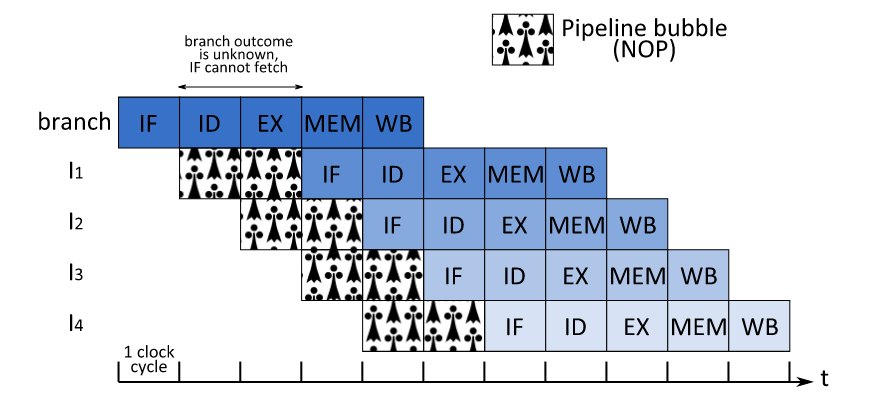
\includegraphics[width=\textwidth]{figures/pipeline-bubbles.png}
    \caption{Example of control hazard: the pipeline is stalled until branch finished the execution (from \cite{perais_increasing_2016})}
    \label{fig:bubbles}
\end{figure}

\subsection{Multiscalar Execution}

Instead of fetching instructions one by one, it is possible to fetch several ones in the same time. This also means that other stages are also multiplied to accommodate all fetched instructions. Since neighbor instructions may be independent this can significantly increase the performance. However, duplicating each stage is costly, while it is relatively easy for IF, ID and COM, execution and accessing memory is much harder to duplicate.

\subsection{Out-of-Order (OoO) Pipeline}

Despite the fact that the instructions are to be processed in program order, many of them are in fact independent. This means that the order of execution can be chosen based on instruction dependencies rather than their order in initial program. Notice that the pipeline is often stalled by the execution of long instructions (\TODO{refer visual example}). The key idea is that while one instruction is being executed on one functional unit (FU), the other, independent of this one can be executed on the other FU. 

In this approach we divide the pipeline into in-order and out-of-order parts. In-order consists of IF, ID and COM stages while out-of-order includes execution and memory accesses. This allows to achieve a consistent ISA-stage due to in-order fetch a commit. 

Different mechanisms exist to synchronize out-of-order execution. Here we introduce reservation stations (RS) and reorder buffer (ROB) - the additional pipeline stages.

Reservation station is a queue before the functional unit, each FU is equipped with its own RS. Once the instruction is decoded it is forwarded to FU based on its type, but if FU is busy, the instruction is put instead into the corresponding RS. Subsequently, the FU is taking the instructions both from ID and RS based on the scheduling policy.

ROB is a FIFO queue that insures the order in which instructions should be committed. Each time, the instruction enters out-of-order part (RS or FU) it is also appended to the front of ROB. After being executed, the instruction is tagged as ready in the ROB. The COM stage commits only the last instruction (or several if multiscalar) from the ROB if it is ready, thus ensuring commit in program order.

\TODO{Image}

\subsection{Branch Prediction}

IF stage is responsible for fetching the next instruction in the program. However, when conditional jump instruction is fetched the next read address is undefined until the outcome of condition is calculated. The straightforward approach is to stall the pipeline, introducing so-called bubbles (no operation).

The more advanced approach consists of fetching a new instruction anyway, the address of which is guessed by branch prediction mechanism, discussed further. Such instructions are called speculative and are not committed until branch decision is taken. In case of incorrect prediction speculative instruction are flushed from the pipeline. 

\section{Branch Predictor Implementations}

\subsection{Static Branch Predictors}

Static branch prediction relies on information known at compile time. Some well-known static branch predictors are:

\begin{itemize}
    \item Always Not Taken
    \item Always Taken
    \item Backward Taken, Forward Not Taken
\end{itemize}

\TODO{add details}

\subsection{Dynamic Branch Predictors}

Dynamic Branch Predictors rely on information retrieved from execution and are usually based on previous branch outcomes. The usage of dynamic branch predictors requires additional hardware components which are discussed below.

\textbf{Pattern History Table (PHT)} is used to store information about each branch. It can be a bit denoting whether the branch was taken last time, or a more complex data. PHT is usually indexed by the lower bits of branch instruction address.

\textbf{Branch Target Buffer (BTB)} stores the destinations of previously computed branch. When starting speculative execution, values from BTB are used.

\textbf{Return Stack Buffer (RSB)} is used to predict the outcome of \textit{ret} instructions.

\subsubsection{One-Bit Predictor}

The one-bit predictor is the simplest type of dynamic branch predictor. It uses PHT indexed by lower bits of address where one-bit value encodes the last branch outcome. Such a simple predictor is efficient when branch decision is not often changed throughout execution. For example, loop conditions are mispredicted only twice by this type of predictor: on the first and the last iterations of the loop.

However, more complex patterns diminish the efficiency of one-bit predictor. For instance, if branch outcome changes each time, the predictor accuracy is zero.

\subsubsection{Two-Bit Predictor}

The two-bit predictor uses the same idea of PHT-indexing, but instead of storing just the outcome of previous branch, it has 4-state automaton encoded by 2 bits. The states are STRONG-TAKEN, WEAK-TAKEN, WEAK-NTAKEN and STRONG-NTAKEN. Picture \TODO{} shows the transitions between the states.

\begin{figure}
    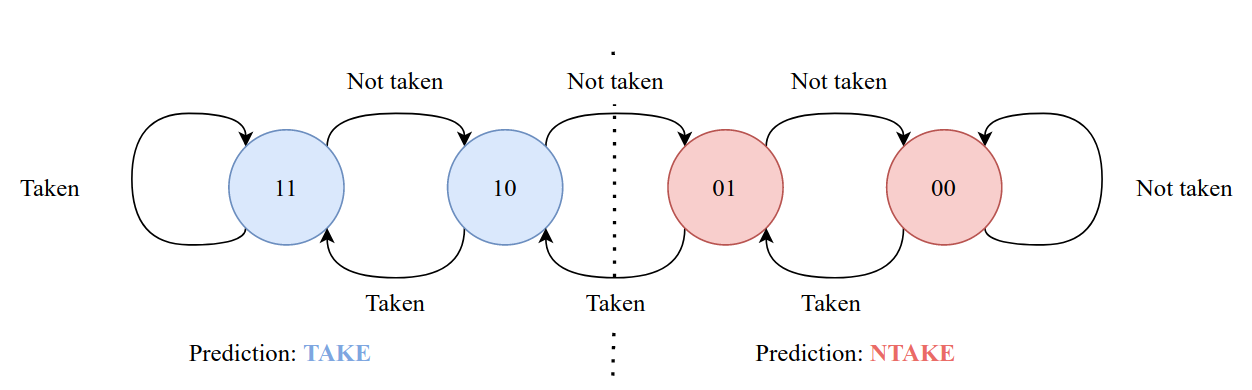
\includegraphics[width=\textwidth]{figures/two-bit-counter.png}
    \label{fig:two-bit-counter}
    \caption{Two-bit predictor state machine (from \cite{mahling_reverse_2023})}
\end{figure}

\TODO{why better than 1-bit}

\TODO{other types. which are used in critical systems?}


\section{WCET Analysis}

In critical systems such as \TODO{examples} it is important that the tasks executed on the hardware meet their deadlines. This is ensured by worst execution time (WCET) analysis. It takes the pair of the program and the dedicated hardware and aims at giving an upper-bound on execution time. 

\TODO{stages of WCET-analysis}

\section{Timing Anomalies}

Phase ordering is a major chellange in WCET-analysis. Most of analysis steps require information from each other (\TODO{examples}), so it is not always possible to order them. 

Nevertheless, most architectures are not composable and contain so-called timing anomalies (TA). Intuitively, TA happens when local worst cases do not constitute a global worst case. TA is observed on the pair of execution traces where the initial hardware state differs, and the instruction sequences are identical. Different cache states can be the source of variation in timing behavior due to miss in one trace and hit in another one.

\begin{example}
Figure \ref{fig:TA1} shows the example of such an anomaly. Here, the assembly sequence consists of 4 instructions ($A,B,C,D$) with data dependencies $A \rightarrow B$ and $C \rightarrow D$. Figure \ref{fig:TA1-trace} represents the pair of traces ($\alpha, \beta$) derived from execution of the given program. There is a variation in latency of instruction $A$ ($1$ in $\alpha$ and $2$ in $\beta$). In trace $\alpha$  the variation is favorable, but the total execution time is also higher in this trace which signals an anomaly.

\label{ex:simple-ta}
\end{example}

\begin{figure}[htbp]
    \centering
    \begin{subfigure}[t]{0.3\textwidth}
        \centering
        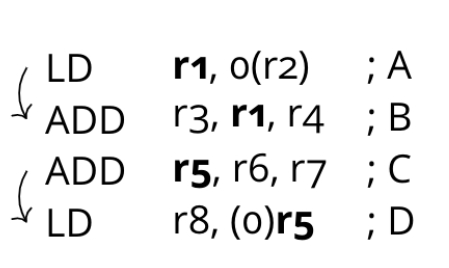
\includegraphics[width=\textwidth]{figures/first-TA-ex-input.png}
        \caption{Inpus assembly sequence}
        \label{fig:TA1-code}
    \end{subfigure}
    \hfill
    \begin{subfigure}[t]{0.55\textwidth}
        \centering
        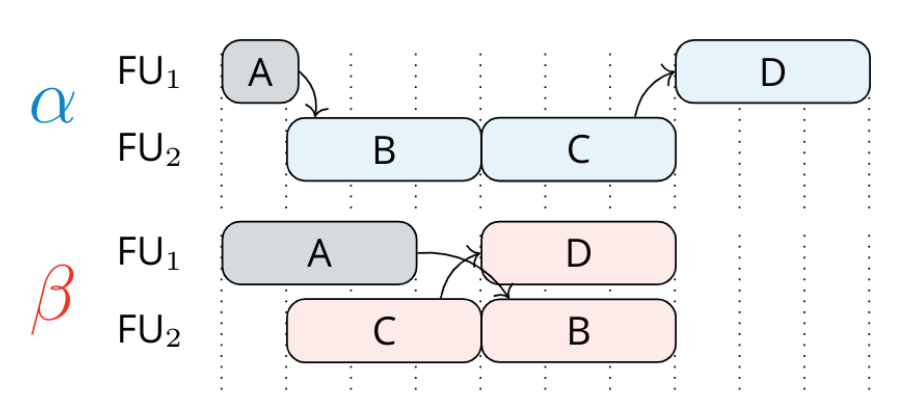
\includegraphics[width=\textwidth]{figures/first-TA-ex-trace.png}
        \caption{Scheduling on functional units comparison}
        \label{fig:TA1-trace}
    \end{subfigure}
    \caption{TA caused by variation in latency of instruction \textit{A} (from \cite{binder_definitions_2022})}
    \label{fig:TA1}
\end{figure}

non-composable architectures

amplification and counter-intuitive TAs

\section{Execution diagrams}

\begin{figure}[htbp]
    \centering
    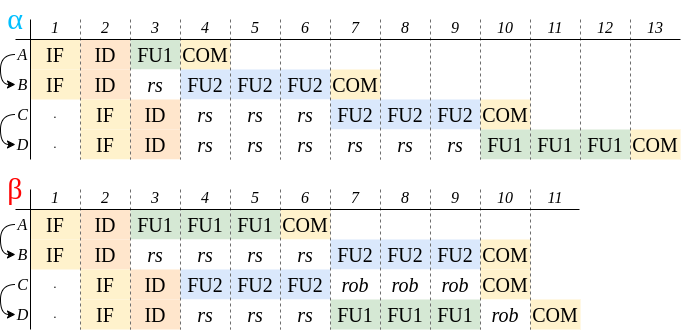
\includegraphics[width=0.8\textwidth]{figures/multiscalar_ta.png}
    \caption{Execution traces from example \ref{ex:simple-ta}}
    \label{fig:multiscalar-ta}
\end{figure}

\TODO{what is trace, what is variation}
\TODO{vertical diagram}
\TODO{diagonal diagram}



\chapter{Timing Analysis and Anomalies}

\section{Evolution of TA-definitions}

A timing anomaly (TA) is a situation where a local favorable condition leads to a globally worse state (for example, a cache hit leading to slowdown of the program).  The notion of timing anomalies dates back to 1999 when they were first introduced by Lundqvist and Stenstr\"om \cite{lundqvist_timing_1999} in context of timing analysis. Basically, TA is a feature of an architecture which makes it hard to analyze timing behavior properly. Such anomalies may have a tremendous impact on execution time which is not captured by the WET analysis. Especially dangerous is so-called domino effect, also discovered by Lundqvist and Stenstr\"om. It leads to an unbounded slowdown effect of the TA.

Despite the fact that timing anomalies have been known for a long time, the exact TA definition is a subject to debates. Since 1999 several attempts were made to formalize the notion of TA, some of them being more focused on the exact microarchitecture (like \cite{gruin_minotaur_2023}) and some being more abstract and general (like \cite{binder_definitions_2022}, \cite{hahn_design_2020}). In this section we are giving an overview of existing definitions comparing their strengths and weaknesses.

\subsection{Step Heights}

Gebhard \cite{gebhard_timing_2012} gives a timing-anomaly definition based on local execution time of instructions in comparison to global execution time defined as sum of local ones. A TA exists when local execution time of earlier instruction is lower and the global execution time of some later instruction is higher (compared to other trace).

Figure \ref{fig:step-good} shows this definition applied to example \ref{ex:simple-ta}. Orange arrow illustrates the local execution time of instruction $A$. The global time for instruction $D$ is different between traces $\alpha$ and $\beta$ (13 and 11 respectively).

\begin{figure}[!htb]
    \centering
    \begin{subfigure}[t]{0.5\textwidth}
        \centering
        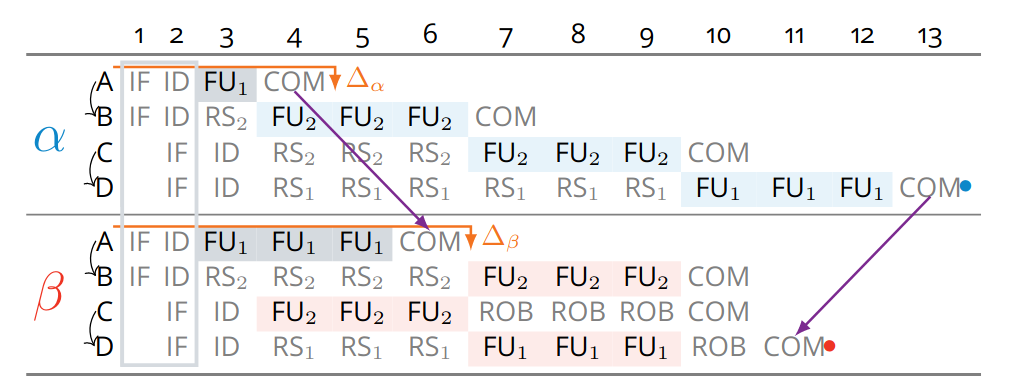
\includegraphics[width=\textwidth]{figures/step-func-good.png}
        \caption{Interpretation of example \ref{ex:simple-ta} using Gebhard's definition}
        \label{fig:step-good}
    \end{subfigure}
    \hfill
    \begin{subfigure}[t]{0.49\textwidth}
        \centering
        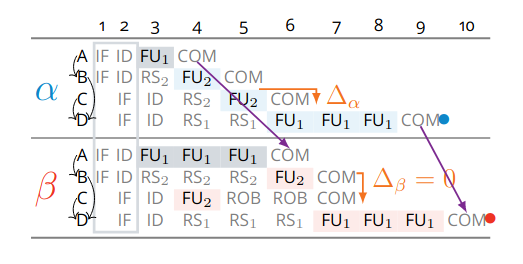
\includegraphics[width=\textwidth]{figures/step-func-bad.png}
        \caption{Counterexample to the definition}
        \label{fig:step-bad}
    \end{subfigure}
    \caption{Gebhard's definition applied to execution traces (from \cite{binder_definitions_2022})}
    \label{fig:step}
\end{figure}

In his thesis \cite{binder_definitions_2022}, Binder provides a counterexample (figure \ref{fig:step-bad}), where it is clear that there is no TA (trace $\beta$ has both unfavorable variation and longer execution time). However, Gebhard's definition signals an anomaly because of shorter local execution time of instruction $C$ in trace $\beta$.

This poses a question whether it is reasonable to capture a local execution time as difference between instruction completion times. 

\subsection{Step-functions Intersections}

Similar definition is proposed by Cassez et al. \cite{cassez_what_2012}. The difference is that only global execution time is taken into account. Thus, TA arises when step-functions (that map instructions to their absolute completion time) of two traces intersect. 

\begin{figure}[!htb]
    \centering
    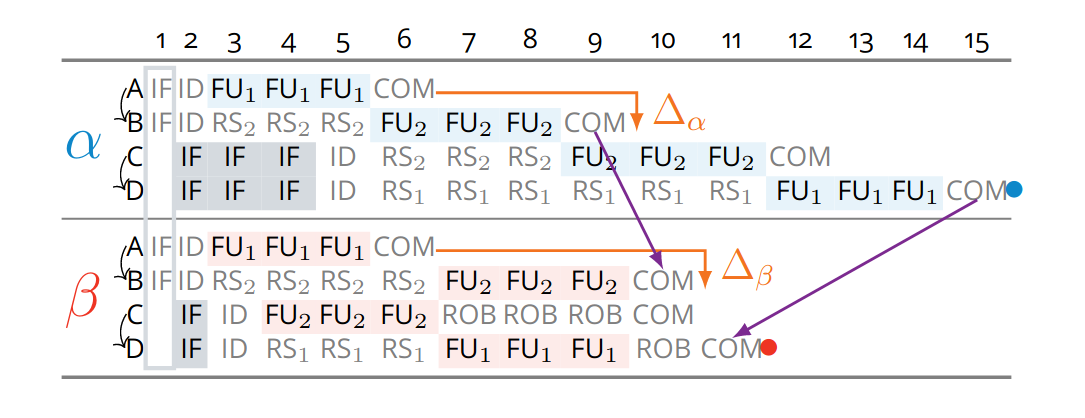
\includegraphics[width=\textwidth]{figures/step-func-2-bad.png}
    \caption{Contradicting result of Cassez's definition (from \cite{binder_definitions_2022})}
    \label{fig:step-2}
\end{figure}

This definition also leads to misleading effect with scenario found by Binder \cite{binder_definitions_2022}. Figure \ref{fig:step-2} illustrates this by comparing two traces. Step-functions of traces $\alpha$ and $\beta$ intersect, however there is no counter-intuitive TA happening as $\alpha$ is both longer and has a  longer latency for IF stage of instructions $C$ and $D$.

\subsection{Component Occupation}

An alternative approach is proposed by Kirner et al. \cite{kirner_precise_2009}. In their work the idea is to partition hardware into components and for each define the occupation by instruction (for how many cycles it processes the instruction). TA arises when a shorter component occupation coincides with a longer execution time in a chosen trace. However, as is shown is \cite{binder_definitions_2022} the results depend on how we define component partition which imposes the major concern against using this definition.

\TODO{counterexample}

\subsection{Instruction Locality}
\subsection{Progress-based definition}

Hahn and Reineke \cite{hahn_design_2020} introduce the notion of progress, ... \cite{gruin_minotaur_2023}

\subsection{Event Time Dependency Graph}

Binder et al. \cite{binder_definitions_2022} define TAs using the notion of causality between events in execution trace. In this work, multiscalar OoO pipeline is considered. The processor state is described as a composition of states of each of the resource: \textit{IF, ID, set of RS, set of FU, ROB, COM}. Each component holds the information about instruction it is currently processing, including required registers and remaining clock cycles.

Notion of event is introduced based on qualitative changes in the pipeline associated to instruction progressing through stages. Event from execution trace (denoted as $e \in Events(\alpha$)) is a triple $(i,r,t)$, where $i$ is the instruction to which event is related, $r$ is the associated resource and the action (acquisition or release) and $t$ is a timestamp corresponding to the clock cycle when event occurs.

In the proposed framework events are related to \textit{IF, ID, FU} and \textit{COM} stages. For each instruction there are 7 types of events: $\IFa$, $\IFr$, $\IDa$, $\IDr$, $\FUa$, $\FUr$ and $COM$. $\uparrow$ signs the acquisition of a resource and $\downarrow$ its release. $COM$ denotes the acquisition of the commit stage; hence its release always happens one clock cycle after and no subsequent stages exist, it is not included into framework.

\textbf{Latency} is defined as the time difference between the acquisition and release of a resource. Each instruction passes through the same pipeline stages and is associated with corresponding events. Therefore, for each pair of traces corresponding to the same program, the sets of events differ only in their timestamps or, potentially, in the functional unit (FU) used (although resource switching is not modeled within this framework). Consequently, for each event in one trace, there exists a corresponding event in the other. Formally, this correspondence is defined by the function $CospEvent: Events(\alpha) \rightarrow Events(\beta)$.


A \textbf{variation} signs that the latency in one trace differs from latency of corresponding events in the other trace. On the pair of traces $\alpha$ and $\beta$. The variation is considered favorable for $\alpha$ if the latency in $\alpha$ is smaller than in $\beta$.

Variations are chosen as a source of timing anomalies. They may represent different memory behavior (cache hit or miss) for fetch and memory accesses in FU. Other sources of TA such as memory bus contention or branching are not considered by the framework.

\textbf{Event Time Dependency Graph (ETDG)} of trace $\tau$ denoted as $G(\tau) = (\mathcal{N}, \mathcal{A})$ is composed of a set of nodes $\mathcal{N} = Events(\tau)$ and a set of arcs $\mathcal{A} \subseteq \mathcal{N} \times \mathcal{N} \times \mathbb{N}$. 


Arc is a triple $(e_1, e_2, w)$ written as $e_1 \xrightarrow{w} e_2$ where $e_1$ is the source event node, $e_2$ -- destination node and $w$ is a lower bound of the delay between the two events. The arc means that at least $w$ clock cycles must pass between $e_1$ and $e_2$. 

Arcs are derived from a set of rules:
\begin{enumerate}
    \item \textbf{Order of pipeline stages}
    
    $(I, \IFa, t_0) \xrightarrow{lat_{IF}} (I, \IFr, t_1) \xrightarrow{0} (I, \IDa, t_2) \xrightarrow{1} (I, \IDr, t_3) \xrightarrow{0} (I, \FUa, t_4)  \xrightarrow{lat_{FU}} (I, \FUr, t_5)  \xrightarrow{0} (I, COM, t_6)$

    $lat_{IF}$ and $lat_{FU}$ are the latencies of IF and FU stages respectively.

    \item \textbf{Resource use}
    
    $lat_{IF} = t_1 - t_0$, $lat_{FU} = t_5 - t_4$

    \item \textbf{Instruction order}
    
    In-order part of the pipeline is constrained by instruction order. Thus, for successive instructions $I_1$ and $I_2$:

    $(I_1, RES\uparrow, t) \xrightarrow{0} (I_2, RES\uparrow, t'), RES \in \{IF, ID, COM\}$


    \item \textbf{Data dependencies}
    
    RAW dependency between $I_1$ and $I_2$ (\TODO{dep notation}) restricts the execution order of the instructions:  $(I_1, \FUr, t) \xrightarrow{0} (I_2, \FUa, t')$.
    
    \item \textbf{Resource contention}
    
    Also some instruction can be delayed because of limited resources. For instance, FU contention happens when $I_1$ and $I_2$ use the same FU, and it is busy by $I_1$ at the moment when $I_2$ is ready. This creates $(I_1, \FUr, t) \xrightarrow{0} (I_2, \FUa, t')$. 

    Resource contention can also be caused by reaching the capacity limit of ROB or RS. 
\end{enumerate}

\textbf{Causality graph} is achieved from ETDG by removing unnecessary edges. For each event we keep only the most relevant constraint. Only arcs of the form $e_1 \xrightarrow{e_2.time - e_1.time} e_2$ are left. Also arcs related to variations are excluded.

\textbf{Timing anomaly} is observed on pair of traces $\alpha$ and $\beta$ if there exists a favorable variation in $\alpha$ relative to $\beta$. Let $e_\alpha\downarrow$ and $e_\beta\downarrow$ be the events corresponding to the end of the variation in both traces. If there exist events $e_\alpha$ and $e_\beta$, where $e_\beta = CospEvent(e_\alpha)$ and there is a path in causality graph of $\alpha$ between $e_\alpha\downarrow$ and $e_\alpha$, s.t. $\Delta(e_\beta\downarrow,e_\beta) < \Delta(e_\alpha\downarrow,e_\alpha)$.


\begin{figure}[htbp]
    \centering
    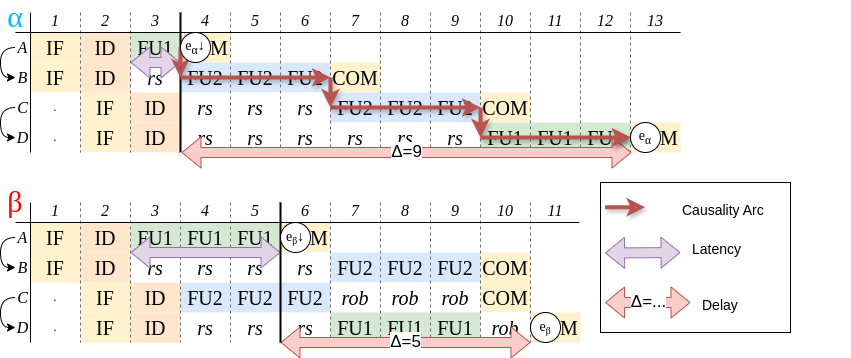
\includegraphics[width=0.8\textwidth]{figures/multiscalar_ta_causality.png}
    \caption{Causality-based TA detection applied to Example \ref{ex:simple-ta}. $e_\alpha\downarrow = (A, \FUr, 4), e_\beta\downarrow = (A, \FUr, 6), e_\alpha = (A, COM, 13), e_\beta = (A, COM, 11)$. Purple arrow denotes latency which has a variation between two traces. Gray arrow shows delay between events which is greater in favorable trace. Causality in  path $\alpha$ is marked by red arrows.}
    \label{fig:multiscalar-ta-causality}
\end{figure}

\begin{figure}[htbp]
    \centering
    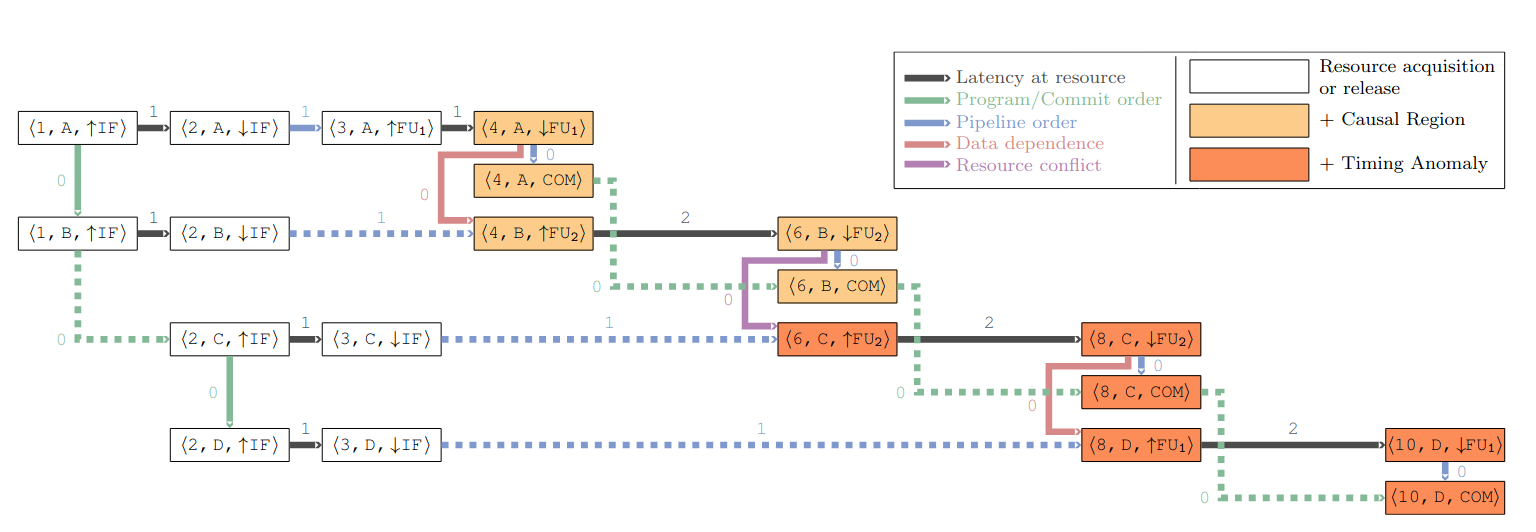
\includegraphics[width=\textwidth]{figures/ETDG.png}
    \caption{Complete ETDG for trace $\alpha$ from figure \ref{fig:multiscalar-ta}. \TODO{image source}}
    \label{fig:ETDG}
\end{figure}

Figure \ref{fig:multiscalar-ta-causality} shows how the framework captures TA for example \ref{ex:simple-ta}. Figure \ref{fig:ETDG} presents the complete ETDG for trace $\alpha$ with different dependency rules highlighted with different colors. The arcs reflecting causality are depicted in solid lines.

In contrast to other definition, this one measures relative time from the acquisition of the resource instead of global time. This approach allows the separation of different variations and isolates the part of the trace that experiences TA-effect.


\section{TA-classifications}


\chapter{Contribution}

\subsection{Input trace format}

\subsection{Adapting definition of Binder et al.}

\subsection{Gap problem}

\subsection{New causality definition}

\subsection{Methodology}

\subsection{Results}

put examples of different TA here
\chapter{Conclusion}

In this report, we have analyzed several existing definitions of timing anomalies (TAs) and, after careful consideration, have chosen to proceed with the definition proposed by Binder et al.~\cite{binder_definitions_2022} as the basis for our study. Consequently, we developed a tool to investigate timing anomalies (TAs) induced by branch prediction. This tool enables the systematic construction and analysis of representative examples. Using this tool, we demonstrated that the definition proposed by Binder et al.~\cite{binder_definitions_2022}, based on variation and causality, and identified as the most prominent among existing definitions, can be adapted to scenarios involving branch prediction. However, our analysis revealed controversial cases that challenge whether Binder's notion of causality fully captures the intuitive understanding of causality in this context. Notably, one issue with Binder's definition, which we refer to as the gap problem, is present even in the original framework and is not specific to branch prediction only. Therefore, further investigation into the aspect of causality is required.

We are currently developing an alternative causality definition based on the notion of constraints for events in the trace. Our approach interprets a change in a constraint as a variation and derives causality links from the resolution procedure, which incrementally adapts the trace to updated constraints. Preliminary evidence suggests that this approach addresses the gap problem.

Also, there are several features that we did not implement in the current tool, such as a shared memory bus model and limitations on the reservation station (RS) and reorder buffer (ROB). These extensions could be incorporated with minimal changes to the tool. Additionally, we did not address the effects of multiple TAs or how effectively their impacts can be separated using the current definition. However, given the lack of a consistent definition, it is premature to pursue this direction.

Another important aspect not addressed by our model is the state of the branch predictor. In our approach, prediction and misprediction are treated as black-box events, similar to how we abstract cache-induced latencies as non-deterministic. While this abstraction simplifies the model, it overlooks the potential to explicitly represent the branch predictor state. As discussed in Chapter~\ref{chap:proc-arch}, branch predictor requires additional hardware features, such as Pattern History Tables (PHT) and Branch Target Buffers (BTB). They could be modeled as part of the pipeline state, allowing us to consider related events in greater detail. This extension could provide deeper insights into how branch decisions propagate through the system and enable us to study not only individual prediction or misprediction events, but also sequences of such events, potentially revealing new types of timing anomalies.

%=========================================================


%=========================================================
\backmatter

\bibliographystyle{plain} % plain-fr si rapport en français 
\bibliography{bibfile.bib}

% \appendix \chapter{Appendix} 

Appendix goes here...

%\cleardoublepage % Goes to an odd page
%\pagestyle{empty} % no page number
%~\newpage % goes to a new even page

\end{document}